\section{Introduction}
As a fundamental problem in computer vision, semantic segmentation aims to assign a semantic class label to each pixel in an image.
Conventional methods rely on stacking local convolution kernel~\cite{long2015fully} to perceive the long-range structure information of the image.

Since the introduction of Vision Transformers~\cite{dosovitskiy2020image}, the landscape of semantic segmentation has significantly revolutionized. 
Transformer-based approaches~\cite{zheng2021rethinking, xie2021segformer} have remarkably demonstrated the capability of global context modeling.
However, the computational cost and memory requirement of Transformer render these methods unsuitable on mobile devices, especially for high-resolution imagery inputs.

Following conventional wisdom of efficient operation, local/window-based attention~\cite{luong2015effective,liu2021swin,huang2021shuffle,yuan2021hrformer}, Axial attention~\cite{huang2019ccnet,ho2019axial,wang2020axial}, dynamic graph message passing~\cite{zhang2020dynamic,zhang2022dynamic} and some lightweight attention mechanisms~\cite{hou2020strip,li2021towards,li2021global,li2020improving,liu2018generating,shen2021efficient,xu2021co,cao2019gcnet,woo2018cbam,wang2020linformer,choromanski2020rethinking,chen2017rethinking,mehta2021mobilevit} are introduced. 

\begin{figure*}
% \vspace{-0.7cm}
    \centering
    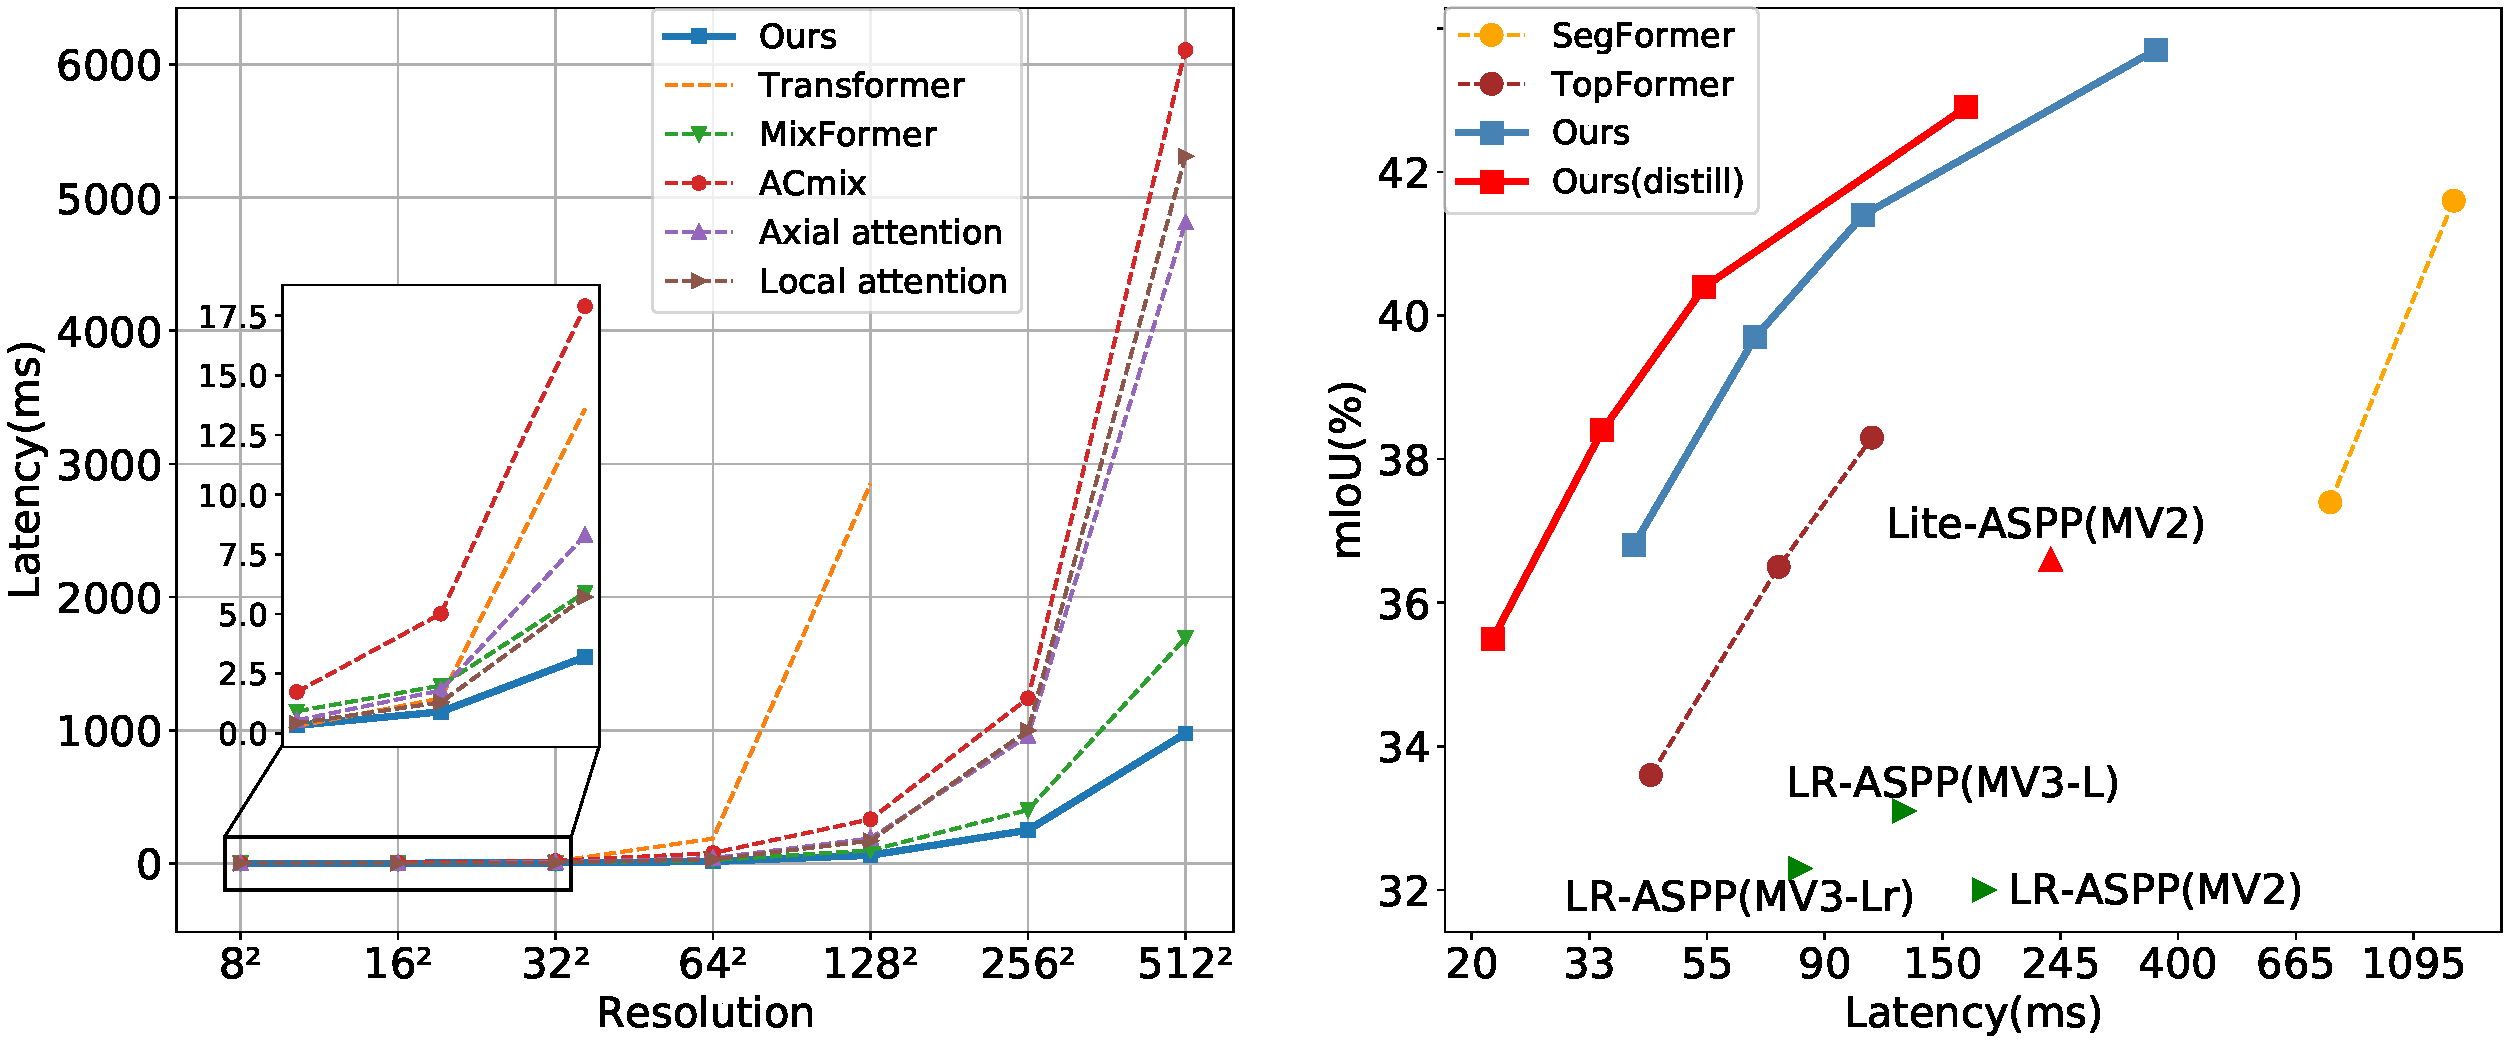
\includegraphics[width=\linewidth]{latency_vs_pixel2.pdf}
    \caption{\textit{\textbf{Left}}: 
    Latency comparison with Transformer~\cite{vaswani2017attention}, MixFormer~\cite{chen2022mixformer}, ACmix~\cite{pan2022integration}, 
    Axial attention~\cite{ho2019axial} and 
    local attention~\cite{luong2015effective}. 
    It is measured with a single module of channel dimension 64 on a Qualcomm Snapdragon 865 processor. 
    \textit{\textbf{Right}}: 
    The mIoU versus latency on the ADE20K \textit{val} set. 
    MV2 means MobileNetV2~\cite{sandler2018mobilenetv2}. 
    MV3-L means MobileNetV3-Large~\cite{howard2019searching}. 
    MV3-Lr denotes MobileNetV3-Large-reduce~\cite{howard2019searching}. 
    The latency is measured on a single Qualcomm Snapdragon 865, and only an ARM CPU core is used for speed testing. No other means of acceleration, e.g., GPU or quantification, is used. For figure \textit{Right}, the input size is 512×512. SeaFormer achieves superior trade-off between mIoU and latency.}
    \label{fig:latency_comp}
% \vspace{-0.2cm}
\end{figure*}
However, these advances are still insufficient to satisfy the design requirements and constraints for mobile devices due to the high latency on the high-resolution inputs (see Figure~\ref{fig:latency_comp}). 
Recently there is a surge of interest in building a Transformer-based semantic segmentation.
In order to reduce the computation cost at high resolution, 
TopFormer~\cite{zhang2022topformer} dedicates to applying the global attention at a $1/64$ scale of the original input, which definitely harms the segmentation performance.

To solve the dilemma of high-resolution computation for pixel-wise segmentation task and low latency requirement on the mobile device in a performance harmless way, we propose a family of mobile-friendly Transformer-based semantic segmentation model, dubbed as \textit{squeeze-enhanced Axial Transformer} (SeaFormer), which reduces the computational complexity of axial attention from $\mathcal{O}((H+W)HW)$ to $\mathcal{O}(HW)$, to achieve superior accuracy-efficiency trade-off on mobile devices and fill the vacancy of mobile-friendly efficient Transformer.

The core building block \textit{squeeze-enhanced Axial attention} (SEA attention) seeks to squeeze (pool) the input feature maps along the horizontal/vertical axis into a compact column/row and computes self-attention.
We concatenate query, keys and values to compensate the detail information sacrificed during squeeze and then feed it into a depth-wise convolution layer to enhance local details.

Coupled with a light segmentation head, our design (see Figure~\ref{fig:pipeline}) with the proposed SeaFormer layer in the small-scale feature is capable of conducting high-resolution image semantic segmentation with low latency on the mobile device.
As shown in Figure~\ref{fig:latency_comp}, the proposed SeaFormer outperforms other efficient neural networks on the ADE20K dataset with lower latency. 
In particular, SeaFormer-Base is superior to the lightweight CNN counterpart MobileNetV3 (41.0 \vs 33.1 mIoU) with lower latency (106ms \vs 126ms) on an ARM-based mobile device.

We make the following \textbf{contributions}:
\textbf{(i)}
We introduce a novel {\em squeeze-enhanced Axial Transformer} (SeaFormer) framework for mobile semantic segmentation;
\textbf{(ii)}
Critically, we design a generic attention block characterized by the formulation of squeeze Axial and detail enhancement;
It can be used to create a family of backbone architectures with superior cost-effectiveness;
\textbf{(iii)}
We show top performance on the ADE20K and Cityscapes datasets, beating both the mobile-friendly rival and Transformer-based segmentation model with clear margins;
\textbf{(iv)}
Beyond semantic segmentation, we further apply the proposed SeaFormer architecture to 
the image classification problem, demonstrating the potential of serving as a versatile mobile-friendly backbone.


A preliminary version of this work was presented in ICLR 2023~\cite{wan2023seaformer}.
In this paper, we have further extended our conference version as follows:
{\bf (i)} 
We propose an adaptive squeeze and expand method in Squeeze-axial attention, using a learnable mask to map all tokens of query/key/values to a single token in each row and column;
{\bf (ii)} 
We present a feature upsampling based multi-resolution distillation approach, further reducing the inference latency of the proposed framework.